\section{Theorie}
\label{sec:Theorie}
Der für Menschen hörbare Frequenzbereich liegt zwischen ca. $\qty{16}{Hz}$ bis $\qty{20}{kHz}$.
Unterhalb dieses Frequenzbereich wird als Infraschall bezeichnet.
Der Frequenzbereich von $\qty{20}{kHz}$ bis $\qty{1}{GHz}$ wird Ultraschall genannt.
Bei Frequenzen über $\qty{1}{GHz}$ wird dieser Bereich als Hyperschall bezeichnet.\\


\noindent Bei der Doppler-Sonographie wird der sogenannte Doppler-Effekt verwendet.
Der Doppler-Effekt beschreibt die Frequenzänderung, wenn sich die Schallquelle und ein Beobachter relativ zueinander bewegen.
Es lassen sich vier verschiedene Fälle betracheten.
Beim ersten Fall, befindetet sich der Beobachter in Ruhe und die Schallquelle bewegt sich auf den Beobachter zu.
Die Frequenz $\nu_0$ der Quelle verschiebt sich zu einer höheren Frequenz $\nu_\text{gr}$.
Entfernt sich die Quelle vom Beobachter, verschiebt sich die Freqeunz zu einer kleineren Frequenz $\nu_\text{kl}$.
Die verschobenen Frequenzen lassen über 
\begin{equation}
    \label{eq:vklgr}
    \nu_\text{kl/gr} = \frac{\nu_0}{1 \mp \frac{v}{c}}
\end{equation}
berechnen.
Dabei beschreibt v die Geschwindigkeit der Quelle und c die Schallgeschwindigkeit.
Im Fall, dass sich die Quelle in Ruhe befindete und sich der Beobachter sich von der Quelle weg bewegt, verschiebt sich die Frequenz zu einer niedrigeren
Frequenz $\nu_n$.
Wenn der Beobachter sich auf sie zu bewegt, wird die Frequenz zu einer höheren Frequenz $\nu_h$ verschoben.
Berechnet werden diese Verschiebungen mit 
\begin{equation}
    \label{eq:vhn}
    \nu_\text{h/n} = \nu_0 \Bigl(1 \pm \frac{v}{c}\Bigr).
\end{equation}
In der Medizin wird der Doppler-Effekt in der Ultraschalltechnik benutzt.
Beispielsweise lässt sich die Geschwindigkeit von Blutströmungen ermitteln.
Dabei trifft die Ultraschallwelle auf die bewegten Blutkörper.
Die Frequenz verschiebt sich um $\Delta \nu$.
Dies lässt sich berechnen mit 
\begin{equation}
    \label{eq:deltav}
    \Delta \nu = \nu_0 \frac{v}{c}(\cos \alpha + \sin \beta).
\end{equation}
Die Winkel $\alpha$ und $\beta$ beschreiben dabei den Winkel zwischen der Geschwindigkeit v des bewegten Objekts und der Wellennormalen der einlaufenden bzw. auslaufenden Welle.
Das Impul-Echo-Verfahren hat die Besonderheit, dass die beiden Winkel identisch sind und somit $\alpha = \beta$ gilt.
Dies ist auch in der Abbildung \ref{fig:IEV} zu erkennen.
\begin{figure}[H]
    \centering
    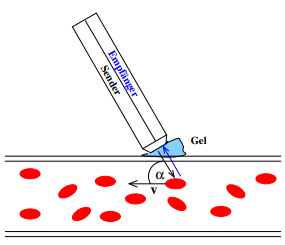
\includegraphics[scale=0.5]{content/TheoBild.png}
    \caption{Blutströmung bestimmen durch das Impuls-Echo-Verfahren \cite{sample}.}
    \label{fig:IEV}
\end{figure}
\noindent Die Winkel sind identisch, da die Ultraschallsonde Sender und der Empfänger enthält.
Die Frequenzverschiebung lässt sich aufgrunddessen berechnen über
\begin{equation}
    \Delta \nu = 2 \nu_0 \frac{v}{c} \cos \alpha.
    \label{eq:deltaf}
\end{equation}
\\

\noindent Um Ultraschallwelle zu erzeugen, kann der reziproken Piezo-elektrischen Effekt verwendet werden.
Dabei wird in ein elektrisches Wechselfeld ein piezoelektrischen Kristall gebracht.
Dadurch wird der Kristall zur Schwingung angeregt und die Ultraschallwellen strahlen vom Kristall ab.
Eine hohe Schallenergiedichte wird erreicht, wenn die Anregungsfrequenz der Eigenfrequenz entspricht.
Es kommt zur Resonanz.
Der piezoelektrische Kristall kann auch als Empfänger verwendet werden.
Dabei treffen die Wellen auf den Kristall, wodurch dieser zur Schwingung angeregt wird.
Am besten eignen sich Quarze als piezoelektrischer Kristall, da die physikalischen Eigenschaften gleich bleiben.

\noindent Damit die Sonde besser an die Oberfläche eines Rohres gekopperlt werden kann, wird ein Doppler-Prisma verwendet.
Dieser bestitzt verschiedene Einschallwinkel, wodurch die Dopplerwinkel $\alpha$ zur strömenden Flüssigkeit repoduzierbar sind.
Diese Dopplerwinkel lassen brechnen über
\begin{equation}
    \alpha = 90° - \arcsin \Bigr( \sin \theta \cdot \frac{c_L}{c_P}\Bigl).
    \label{eq:alp}
\end{equation}
Dabei beschreibt $c_L$ die Schallgeschwindigkeit der Dopplerphantomflüssigkeit, $c_P$ die Schallgeschwindigkeit des Dopplerprismas
und $\theta$ den Einschallwinkel des Doppler-Prismas.

\cite{sample}
